% !TeX program = lualatex
\documentclass[10pt, aspectratio=169]{beamer}
\usepackage{pgfpages}
\usepackage{fontawesome}
\usepackage[english]{babel}
\usepackage[utf8]{inputenc}
\usepackage{graphics}
\usepackage[T1]{fontenc}
\usepackage[]{csquotes}
\usepackage[]{url}

% Bibliography (choose backend according to your preferences)
\usepackage[authordate, natbib, useprefix=true, isbn=false,url=false, doi=false, backend=biber]{biblatex-chicago}  
\bibliography{library.bib}
\setbeamertemplate{bibliography item}[text]

% Size of bibliography entries
\renewcommand*{\bibfont}{\footnotesize}

% new citep command
%\usepackage{fixltx2e}
\newcommand{\cpsh}[2][]{\textsuperscript{\fontsize{6}{6}\textcolor{mzescyan}{[{#1}\citealp[]{#2}]}}}
\newcommand{\cpsl}[2][]{\textsubscript{\fontsize{6}{6}\textcolor{mzescyan}{[{#1}\citealp[]{#2}]}}}
\newcommand{\csh}[2][]{\textsuperscript{\fontsize{6}{6}\textcolor{mzescyan}{[{#1}\citealp[]{#2};}}}
\newcommand{\csl}[2]{\textsubscript{\fontsize{6}{6}\textcolor{mzescyan}{\hphantom{[{#2}}\citealp{#1}]}}}
\newcommand{\cpshl}[3][]{\textcolor{mzescyan}{\rlap{\csh[#1]{#2}}{\csl{#3}{#1}}}}
\newcommand{\cpsm}[2][]{\textcolor{mzescyan}{\fontsize{6}{6} [{#1}\citealp[]{#2}]}}

% new color emphasize commands
\newcommand{\cemph}[1]{\textcolor{mzescyan}{#1}}
\newcommand{\gemph}[1]{\textcolor{mzesgold}{#1}}

% Layout
\mode<presentation>
{
	\usetheme[progressbar=frametitle]{metropolis}
	\useoutertheme[]{metropolis}
	\useinnertheme[]{circles}
	
	
	%remove navigation symbols
	\setbeamertemplate{navigation symbols}{}
	
	% define colors
	\definecolor{mzescyan}{RGB}{0,118,150}
	\definecolor{mzesgold}{RGB}{209,163,84}
	\definecolor{mzesdarkgold}{RGB}{127, 110, 87}
	\definecolor{mzesbg}{RGB}{255,255,255} % white
	% \definecolor{mzesbg}{RGB}{252,253,254} % grayish
	
	% Blocks
	\setbeamercolor{block body}{bg=mzescyan!10, fg=black}
	\setbeamercolor{block body alerted}{bg=normal text.bg!90!black}
	\setbeamercolor{block body example}{bg=normal text.bg!90!black}
	\setbeamercolor{block title alerted}{use={normal text,alerted text},fg=mzesgold,bg=black}
	\setbeamercolor{block title}{bg=mzescyan, fg = mzesbg}
	\setbeamercolor{block title example}{use={normal text},fg=example text.fg!75!normal text.fg,bg=normal text.bg!75!black}
	
	% Frames
	\setbeamercolor{fine separation line}{fg=mzesgold}
	\setbeamercolor{item projected}{fg=mzesbg}
	
	% Miniframes
	\setbeamercolor{section in head/foot}{fg=mzescyan,bg=mzesbg}
	
	% Title
	\setbeamercolor{background}{bg=mzesbg}
	\setbeamercolor{background canvas}{bg=mzesbg}
	\setbeamercolor{title}{fg=mzescyan, bg = mzescyan!5}
	\setbeamercolor{titlelike}{fg=mzescyan}
	\setbeamercolor{subsection in head/foot}{bg=mzesgold!10, fg = mzescyan}
	\setbeamercolor{author in head/foot}{bg=mzescyan, fg = mzesbg}
	\setbeamercolor{title in head/foot}{bg=mzescyan!5, fg = mzescyan}
	\setbeamercolor{date in head/foot}{bg=mzesbg, fg = mzescyan}
	\setbeamercolor{page in head/foot}{bg=mzesbg, fg = mzesgold}
	\setbeamercolor{frametitle}{fg=mzescyan, bg = mzesbg}
	\setbeamercolor{item}{fg=mzescyan}
	\setbeamercolor{normal text}{bg=mzesbg,fg=black}
	\setbeamercolor{alerted text}{bg=mzesbg,fg=mzesgold}
	\setbeamercovered{invisible}
}

% Font
\setbeamerfont{frametitle, frametitle continuation}{size=\large}
\setbeamerfont{titlelike}{size=\large}
\setbeamerfont{footline}{size=\scriptsize}

% Logo
\logo{
\includegraphics[width=12em]{mzes-logo-solo-4c.eps}}
\newcommand{\nologo}{\setbeamertemplate{logo}{}}
% customize foot line
\makeatother
\setbeamertemplate{footline}
{
	\leavevmode%
	\hbox{%
		\begin{beamercolorbox}[wd=.25\paperwidth,ht=2.25ex,dp=1ex,center]{author in head/foot}%
			\usebeamerfont{author in head/foot}\insertshortauthor
		\end{beamercolorbox}%
		\begin{beamercolorbox}[wd=.6\paperwidth,ht=2.25ex,dp=1ex,center]{title in head/foot}%
			\usebeamerfont{title in head/foot}\insertshorttitle
		\end{beamercolorbox}%
		\begin{beamercolorbox}[wd=.15\paperwidth,ht=2.25ex,dp=1ex,center]{page in head/foot}%
			\insertframenumber{} / \inserttotalframenumber\hspace*{1ex}
	\end{beamercolorbox}}%
	\vskip0pt%
}
\makeatletter

% Change the width of the progress bar to make it more visible (Code taken from here: https://github.com/matze/mtheme/issues/237)
\makeatletter
\setlength{\metropolis@titleseparator@linewidth}{0.5pt} % Title page
\setlength{\metropolis@progressonsectionpage@linewidth}{1pt} % Progress bar on section page
\setlength{\metropolis@progressinheadfoot@linewidth}{1pt} % Progress bar in header
\makeatother

\setbeamertemplate{navigation symbols}{}
\providecommand*\email[1]{\href{mailto:#1}{#1}}

% title slide
\title[Getting Started with Python] % (optional, use only with long paper titles)
{\large \textbf{Getting Started With Python}} 
\subtitle{\small A \textit{How-To} Guide for Social Scientists}

\author[Bach \& K\"{u}pfer]{%
	\texorpdfstring{
		\begin{columns}
			\begin{column}{0.45\textwidth}
				Ruben Bach \\
				\scriptsize University of Mannheim \vspace{1em} \\
				\tiny \hspace*{1em} \faEnvelope \hspace{.5em} \texttt{\email{r.bach@uni-mannheim.de}} \\
%				\tiny \hspace*{1em} \faGlobe \hspace{.5em}  \texttt{\href{https://denis-cohen.github.io/}{denis-cohen.github.io}} \\
				\tiny \hspace*{1em} \faTwitter \hspace{.5em} \texttt{\href{https://twitter.com/rub3n_luc}{@rub3n\_luc}}
			\end{column}
			\begin{column}{0.45\textwidth}
				Andreas K\"{u}pfer \\
				\scriptsize Technical University of Darmstadt \vspace{1em} \\
				\tiny \hspace*{1em} \faEnvelope \hspace{.5em} \texttt{\email{andreas.kuepfer@tu-darmstadt.de}} \\
				\tiny \hspace*{1em} \faGlobe \hspace{.5em}  \texttt{\href{https://andreaskuepfer.github.io/}{andreaskuepfer.github.io}} \\
				\tiny \hspace*{1em} \faTwitter \hspace{.5em} \texttt{\href{https://twitter.com/}{@ankuepfer}}
			\end{column}
		\end{columns}
	}
	{Bach \& K\"{u}pfer}
}
\date{}
\institute{Social Science Data Lab\\ MZES, University of Mannheim \\ February 15, 2023}
\subject{}



\begin{document}

\begin{frame}
  \titlepage
\end{frame}

\nologo{ % no logos except on the title page
	\begin{frame}{Outline}
		\tableofcontents
	\end{frame}
\section{Why Python?}
	
	\begin{frame}{Why Python?}
  \begin{columns}
\begin{column}{0.5\textwidth}
	\cemph{Python and R can do the same things, e.g., ...}
 \begin{itemize}
                \item Analyze data using regression and machine learning techniques
                \item Collect data from the web, e.g., through scraping and APIs
                \item Visualize data
            \end{itemize}
\end{column}
\begin{column}{0.5\textwidth}  %%<--- here
    \begin{center}
      
\includegraphics[scale=.3]{Day 1/Slides/LaTeX files/why-not-both.jpg} \\
            \tiny{Created with the Imgflip \href{https://imgflip.com/memegenerator}{Meme Generator}}
     \end{center}
\end{column}
\end{columns}
  \end{frame}

	\begin{frame}{Why Python?}
	\small
	\cemph{Python, however, is better suited when ...}
            \begin{itemize}
                \item Working with computer scientists
                \item Using state-of-the-art machine learning, deep learning, natural language processing
                \item Preparing for a data science job outside of academia
                \item General purpose programming
            \end{itemize}
    \small
	Full disclosure: If your work is focused on statistical inference and explanation (coefficients, statistical tests, ...) and some ML and NLP, you'll probably be better-off with R. For prediction-focused ML, deep learning, NLP and heavy data science, you'll probably want to consider using python at some point.
  \end{frame}


\section{Virtual Environments and Packages}
	
	\begin{frame}{Python}
	\small
            \begin{itemize}
                \item General purpose programming language
                \item Three major versions, only one (Python 3) still maintained
                \item Starting today, obvious choice is Python 3
            \end{itemize}
   		\begin{block}{Is python already installed?}
			\$ python --version
		\end{block}       
  \end{frame}

	\begin{frame}{Versioning of python and packages}
	\small
            \begin{itemize}
                \item Installing the most recent stable release of python in your root environment and packages is a good starting point
                \item Sometimes, dependencies require other versions of Python and/or packages, however
                \item Solution: Set up different \cemph{virtual environments} 
                \begin{itemize}
                    \item Easy to keep different versions of Python and packages
                    \item Avoid problems with different dependencies and updates
                    \item Can easily switch between virtual environments
                    \item Makes it easier for your code to run on collaborators' setups
                \end{itemize}
            \end{itemize}     
  \end{frame}

 	\begin{frame}{Creating and maintaining virtual environments}
	\small
 \textbf{With \gemph{PIP} and \gemph{venv}}
\begin{itemize}
    \item \textbf{venv}: Should come with your python installation
    \item Tool to set up and manage virtual environments
\end{itemize}
\vskip .5cm
                \begin{block}{Create a new virtual environment using \gemph{venv}}
                   \$ python -m venv <directory>
		          \end{block}
                
               
                 \begin{block}{Activate virtual environment (Linux/Mac)}
                   \$ source <directory>/bin/activate
		          \end{block} \begin{block}{Activate virtual environment (Windows)}
                   \$ <directory>/Scripts/activate
		          \end{block}
                \begin{block}{Deactivate virtual environment}
                   (<directory>) \$ deactivate
		          \end{block}
        


  \end{frame}

  	\begin{frame}{Versioning of python and packages}
	\small
\textbf{With \gemph{PIP} and \gemph{venv}}
                \begin{itemize}
                    \item \textbf{pip}: \textbf{P}ip \textbf{I}nstalls \textbf{P}ackages
                    \item Standard package manager for python packages
                    \item pip3: specifically installs packages for python 3, can be ignored if you do not have python 2 on your system
                    \item Should come with your python installation
                    \item Install packages within a virtual environment
                \end{itemize}
                \begin{block}{Install \gemph{pip}}
                   \$ python -m ensurepip --upgrade
		          \end{block} 
                \begin{block}{Install packages using \gemph{pip}}
                   \$ pip install <package name>
		          \end{block} 
  \end{frame}

  	\begin{frame}{Versioning of python and packages}
	\small
                 \begin{block}{List installed packages}
                   \$ pip list
		          \end{block} 
                \begin{itemize}
                    \item Sometimes, a \texttt{requirements.txt} file is provided
                    \item Contains required packages and versions
                \end{itemize}
                \begin{block}{Install packages from \gemph{requirements.txt}}
                   \$ pip install -r requirements.txt
		          \end{block} 
            \begin{itemize}
                \item Note
                \begin{itemize}
                    \item Virtual environments are disposable folder structures
                \item Do not put code or data into your virtual environment (folder) manually
                \end{itemize}
            \end{itemize}
  \end{frame}



       	\begin{frame}{Creating and maintaining virtual environments}
\small          
 \gemph{Conda}
\begin{itemize}
    \item "Package, dependency and environment management for any language"
    \item Installation
    \begin{itemize}
        \item Via \cemph{Anaconda}: python (and R) distribution, popular in data science, many pre-installed packages, Anaconda Navigator (GUI)
        \item Via \cemph{miniconda}: Fewer packages than Anaconda, no GUI
        \item Install through \href{https://www.anaconda.com}{Anaconda} website
    \end{itemize}
    \begin{block}{Check if conda has been installed}
                   \$ conda --version
		          \end{block} 
\end{itemize}
  \end{frame}





       	\begin{frame}{Creating and maintaining virtual environments}
\small          
 \gemph{Conda}
 \begin{block}{Create a new virtual environment}
                   \$ conda create --name mynewenv python=3.11

		          \end{block} 
            
                 \begin{block}{Activate virtual environment (Linux/Mac)}
                   \$ source activate mynewenv
		          \end{block} \begin{block}{Activate virtual environment (Windows)}
                   \$ activate mynewenv
		          \end{block}
             \begin{block}{Dectivate virtual environment (Linux/Mac)}
                   \$ source deactivate
		          \end{block}
              \begin{block}{Dectivate virtual environment (Windows)}
                   \$ deactivate
		          \end{block}

  \end{frame}

       	\begin{frame}{Creating and maintaining virtual environments}
\small          
 \begin{block}{List installed packages}
                   \$ conda list

		          \end{block} 
            
                 \begin{block}{Install packages (including version number)}
                   \$ conda install <package name>=0.7.0
		          \end{block} \begin{block}{Update packages (or a specific one)}
                   \$ conda update [<package name>]
		          \end{block}
             Sometimes, a package is not available through \cemph{conda} channels. You could still install it using \cemph{pip}
              \begin{block}{E.g., install package "lightgbm" using pip}
                   \$ pip install lightgbm
		          \end{block}

  \end{frame}


	
	\section{Graphical User Interfaces and Integrated Development Environments}

 
	\begin{frame}{GUIs and IDEs}
		\begin{itemize}
		    \item There is no one-stop shop like RStudio
            \item However, \cemph{Anaconda} and \cemph{Anaconda Navigator} integrate many of the tools for  a Python data science environment
            \begin{itemize}
                \item "Anaconda is a distribution of the Python and R programming languages for scientific computing (data science, machine learning applications, large-scale data processing, predictive analytics, etc.), that aims to simplify package management and deployment. (...) Package versions in Anaconda are managed by the package management system conda" \href{https://en.wikipedia.org/wiki/Anaconda_(Python_distribution)}{Wikipedia}
                \item "It also includes a GUI, Anaconda Navigator, as a graphical alternative to the command-line interface (CLI)."
            \end{itemize}
		\end{itemize}
	\end{frame}

 	\begin{frame}{GUIs and IDEs}
\begin{center}
      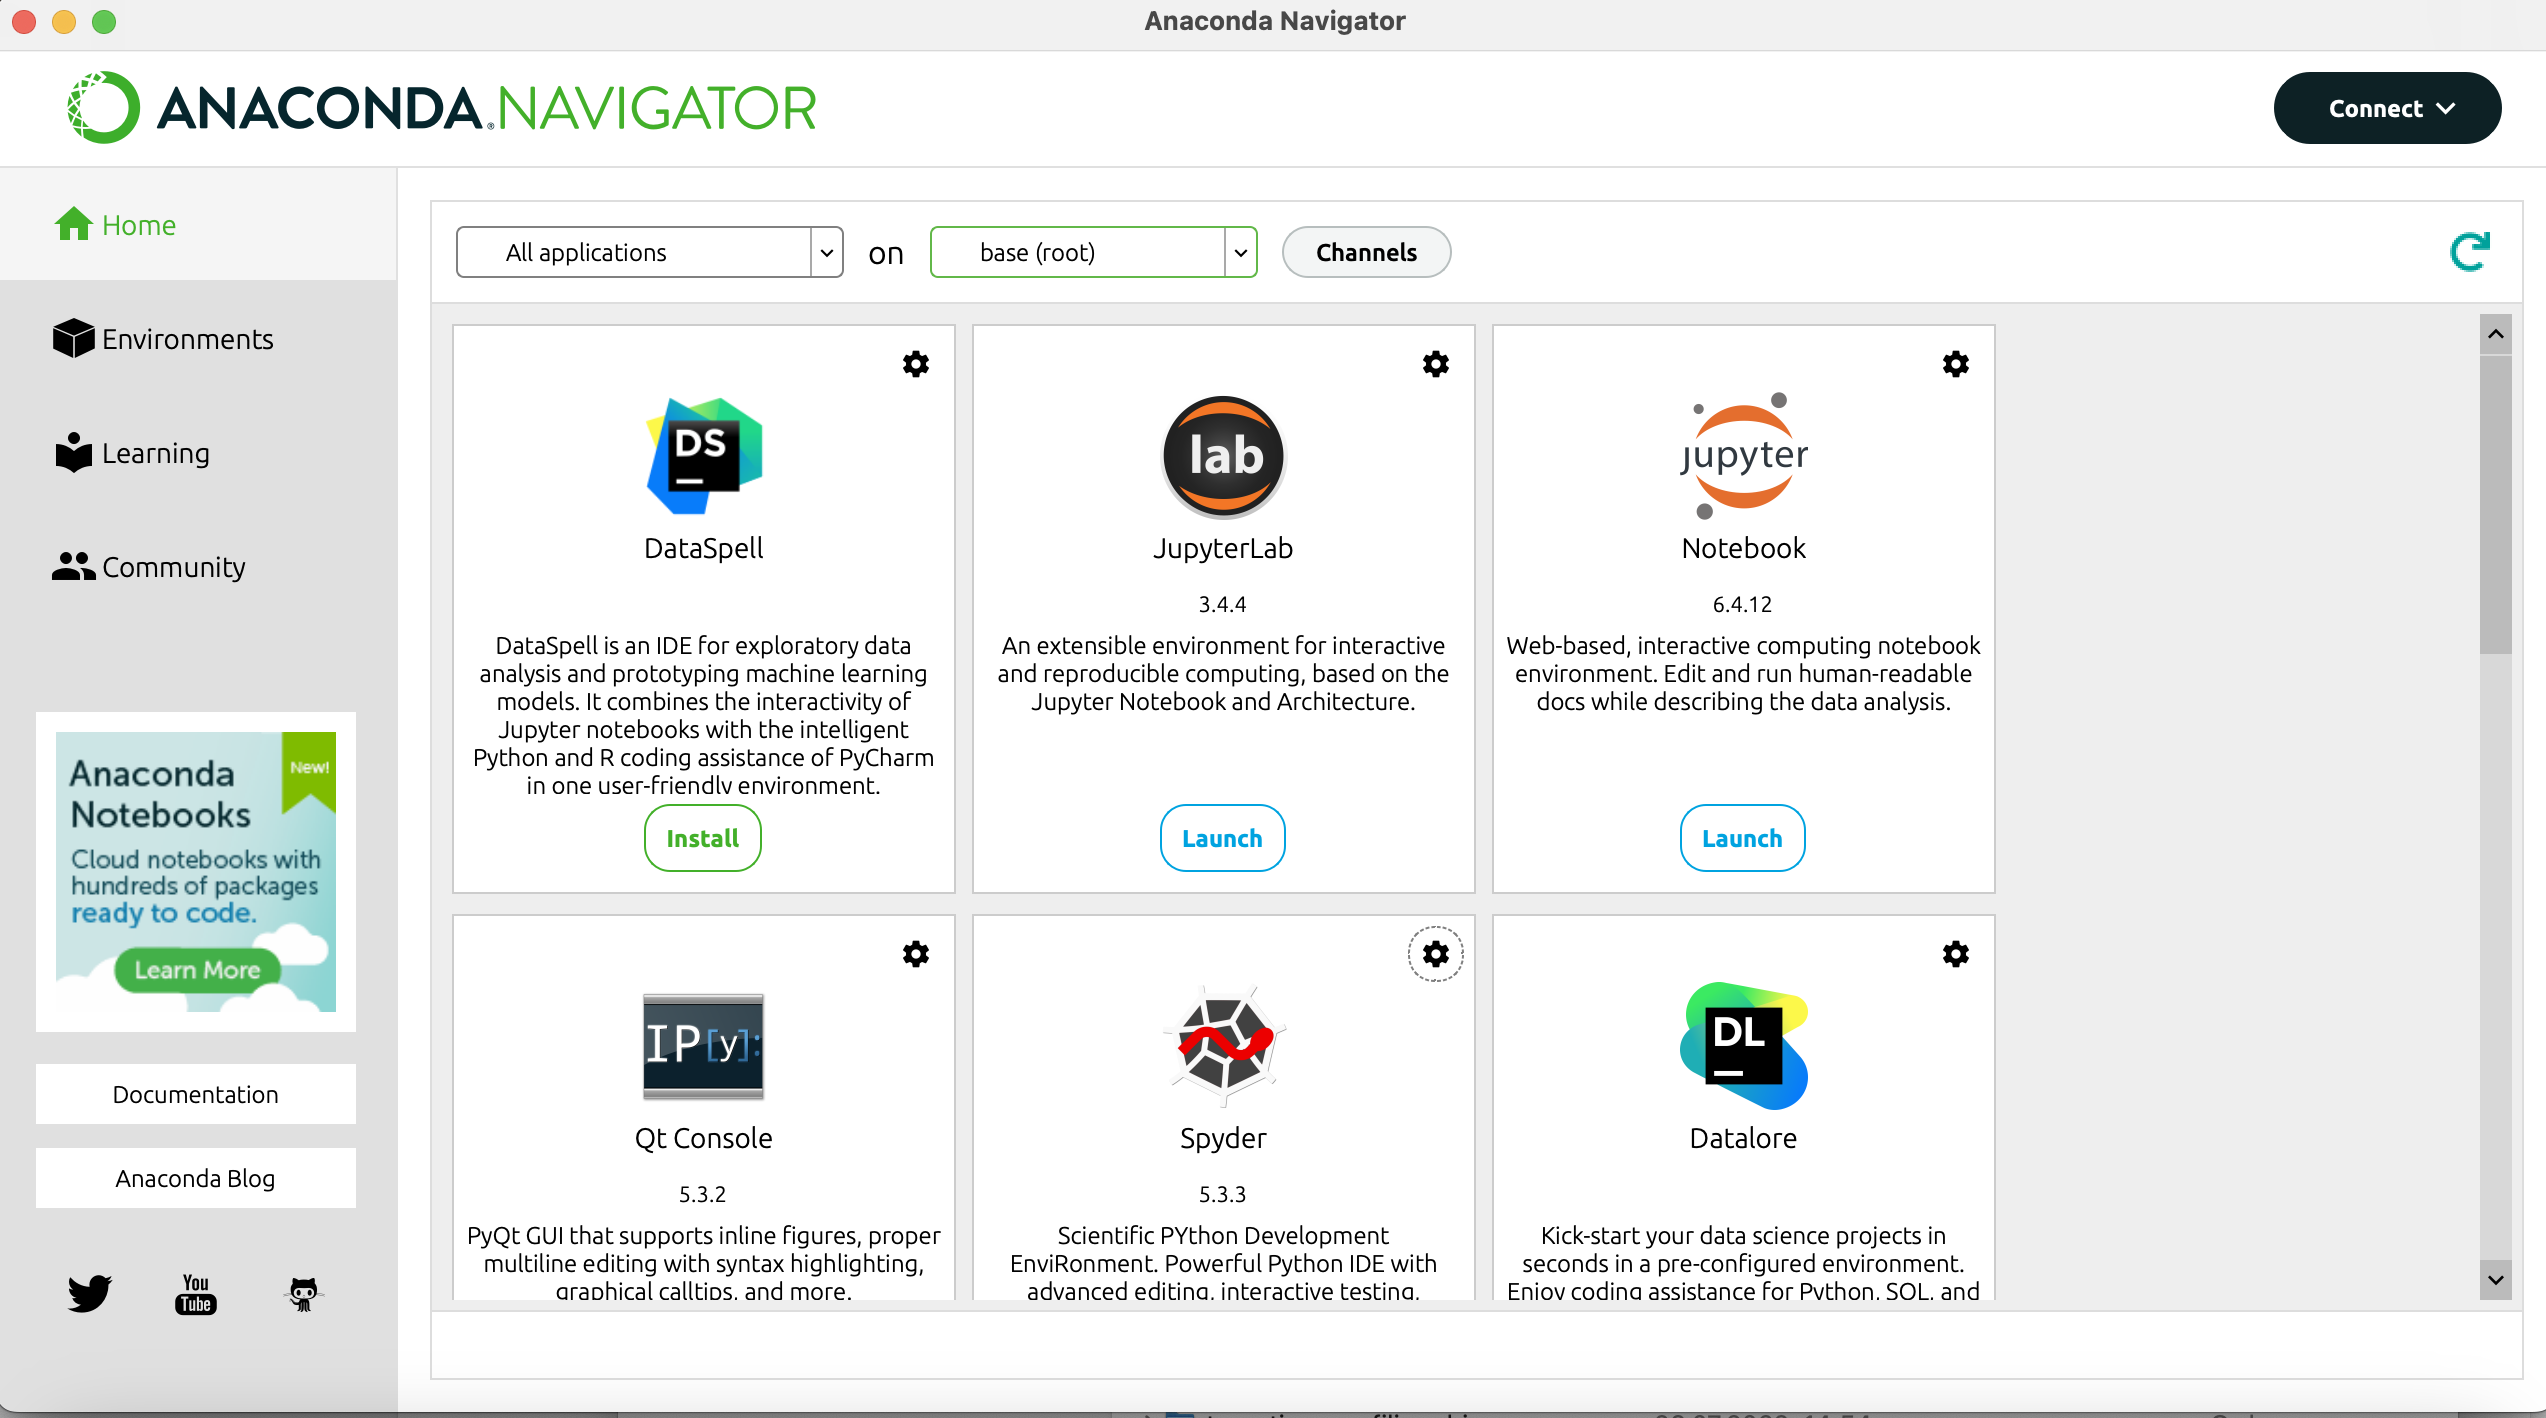
\includegraphics[scale=.28]{Day 1/Slides/LaTeX files/Anaconda-navigator.png} \\
     \end{center}
	\end{frame}

  	\begin{frame}{GUIs and IDEs}
\begin{center}
      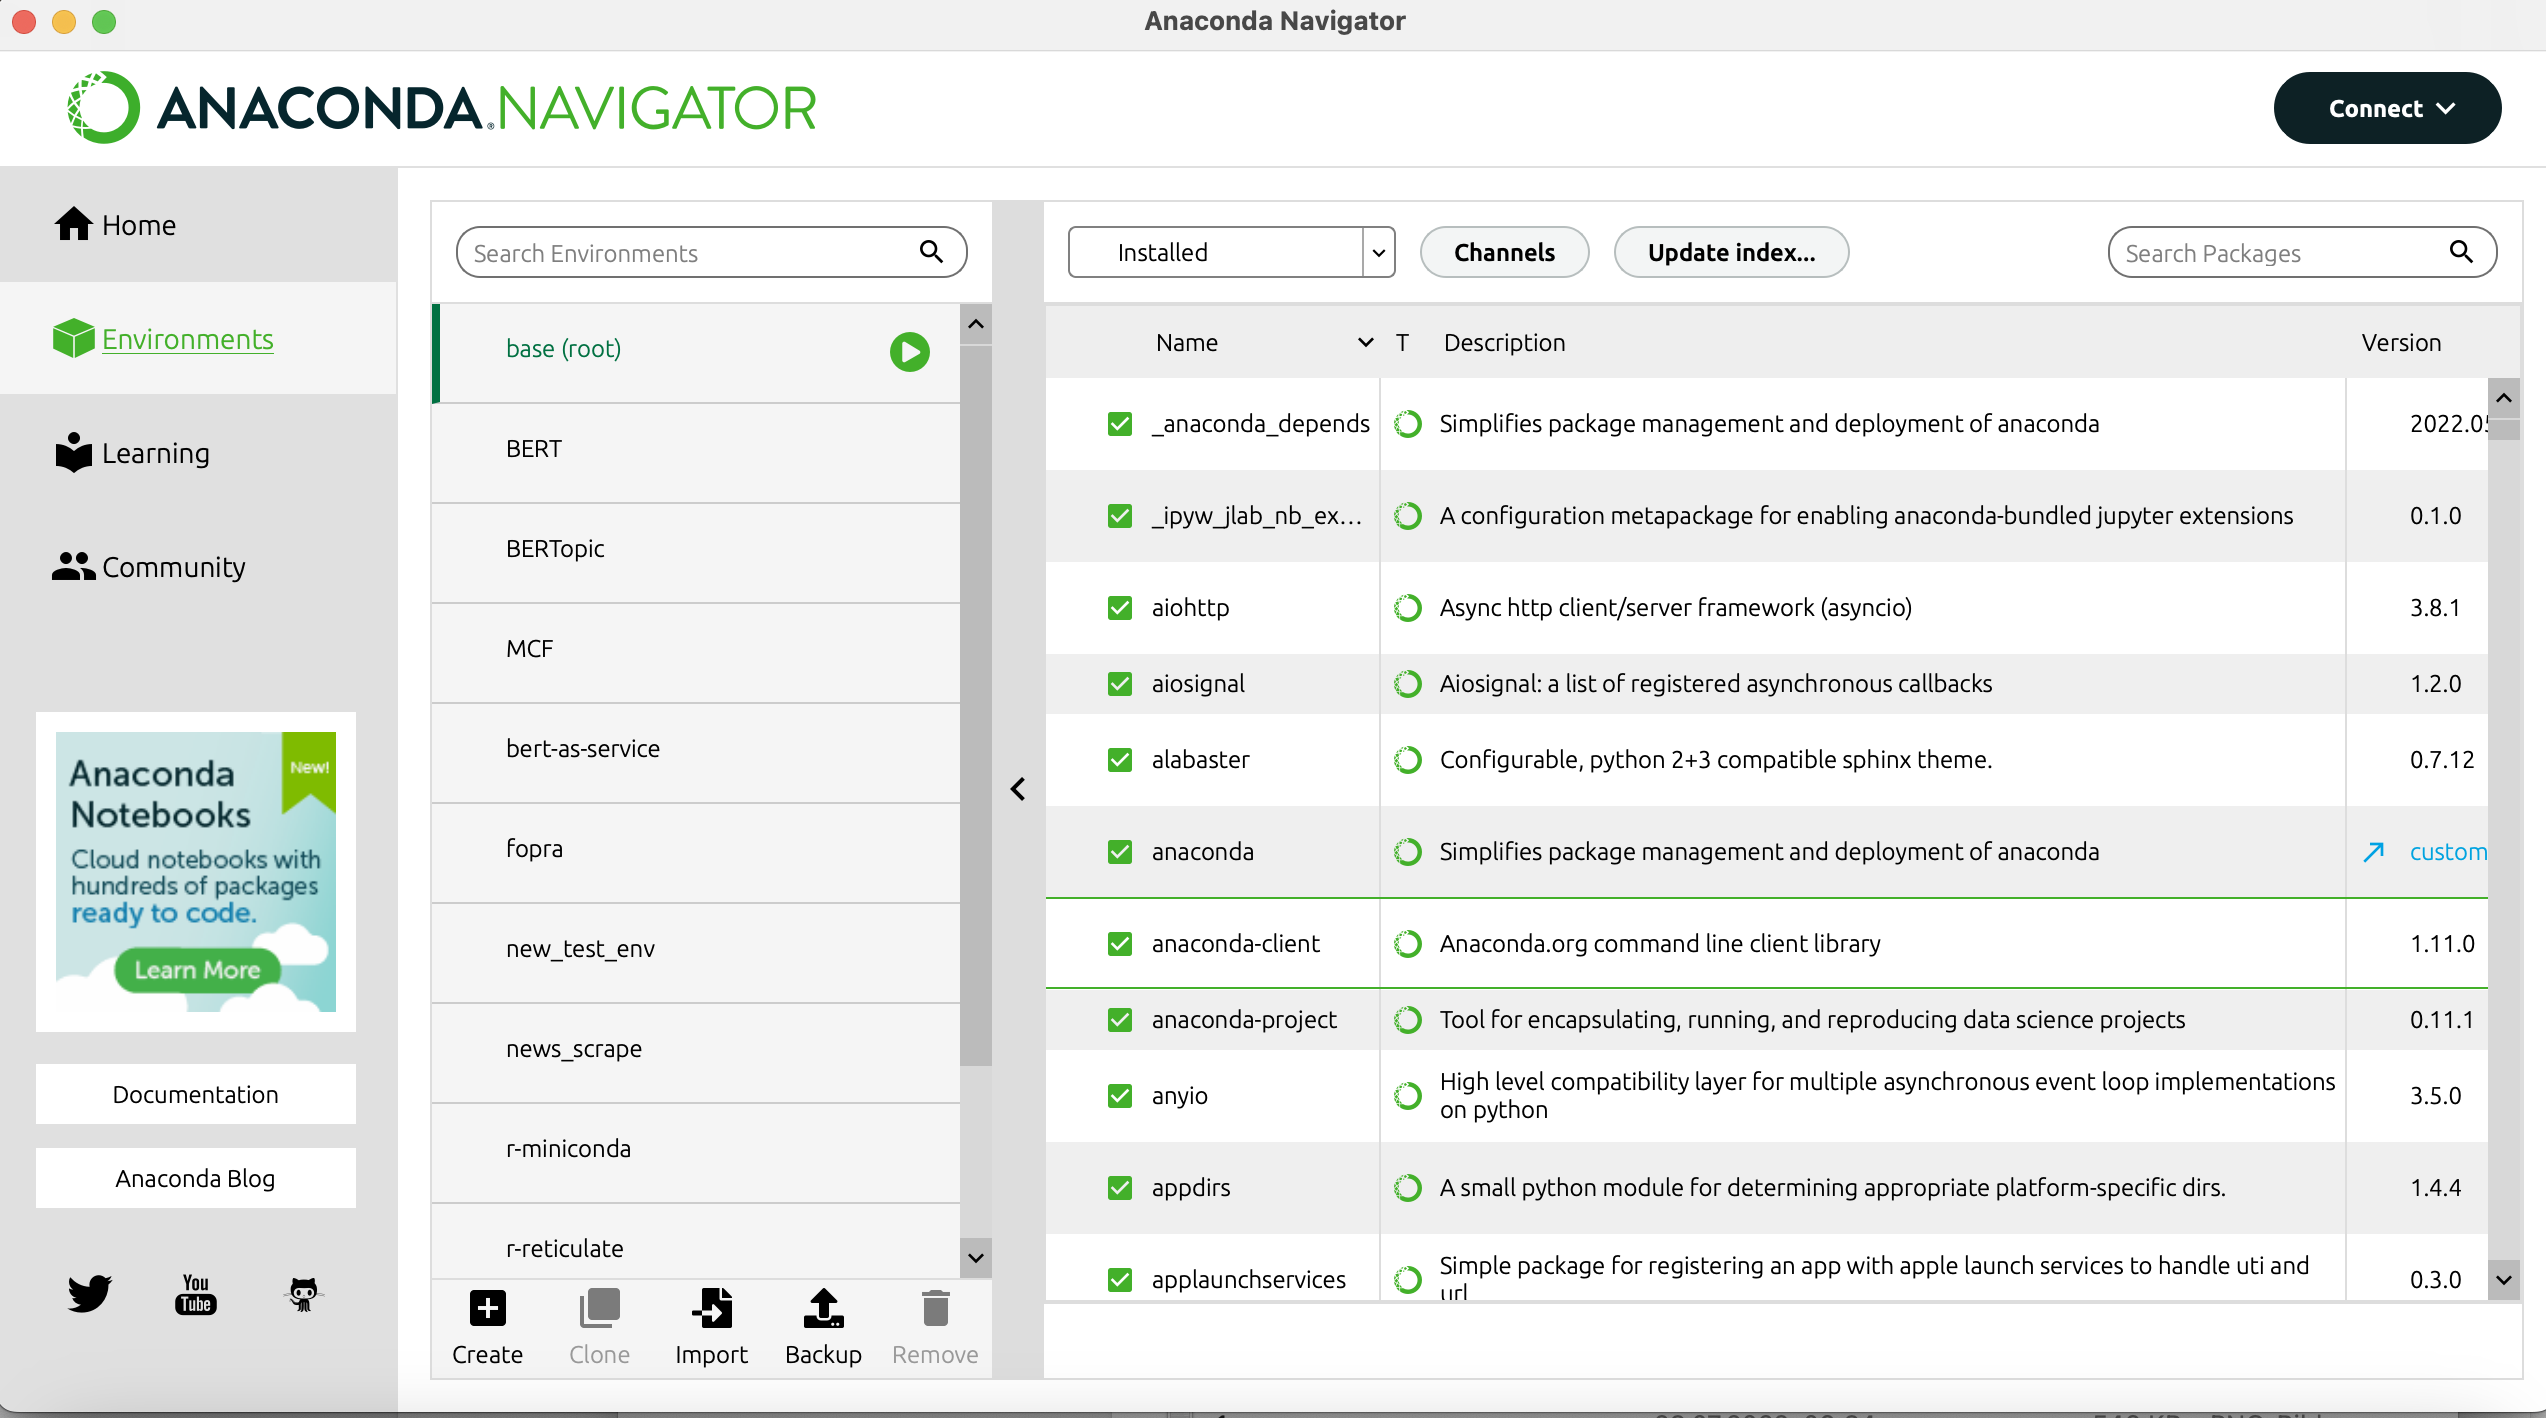
\includegraphics[scale=.28]{Day 1/Slides/LaTeX files/Anaconda-env.png} \\
     \end{center}
	\end{frame}

  	\begin{frame}{IDEs and Notebooks}
\small
Several Integrated Development Environments (IDEs), e.g., ...
\begin{itemize}
    \item Spyder
    \item PyCharm
\end{itemize}
and web-based interactive computing environments like ...
\begin{itemize}
    \item Jupyter Notebook / JupyterLab
    \item Google Colaboratory ("Colab")
\end{itemize}
Note: Unlike in R/RStudio, you will need to install additional packages through a terminal using pip or conda\footnote{Installation through terminal can be sidestepped when using Notebook-type applications.}
\end{frame}

\begin{frame}{Spyder}
    \begin{center}
      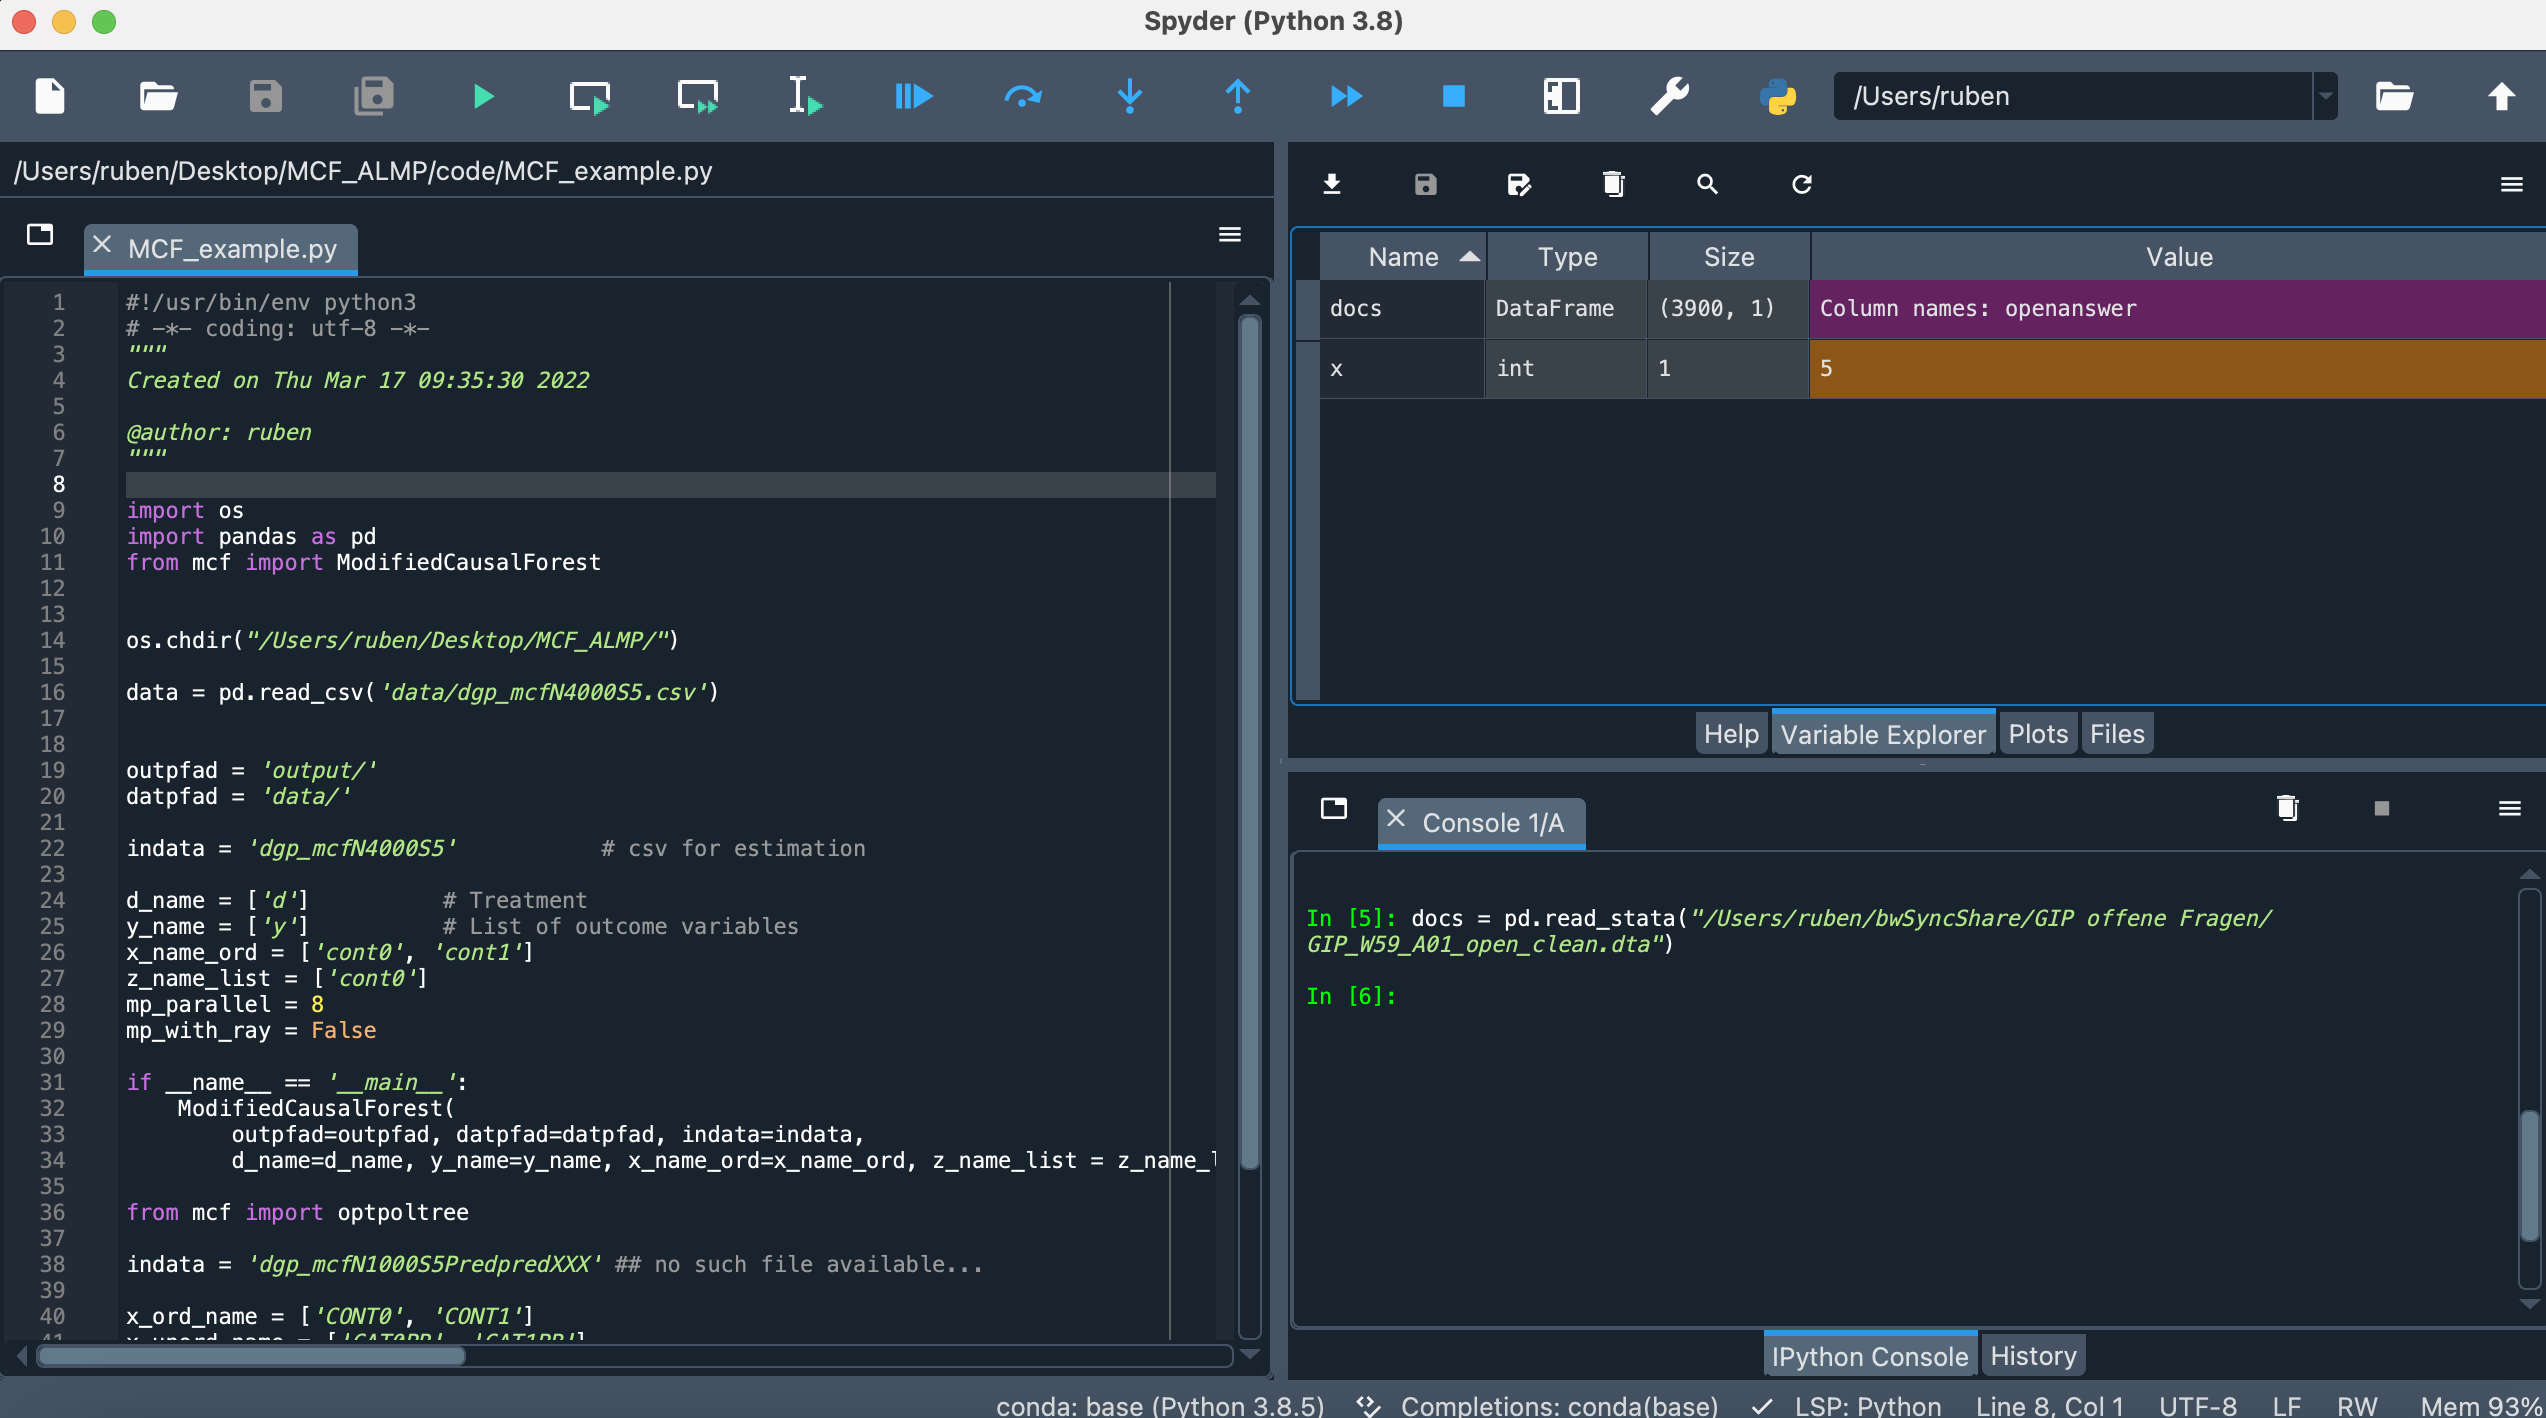
\includegraphics[scale=.28]{Day 1/Slides/LaTeX files/Spyder.png} \\
     \end{center}
\end{frame}

\begin{frame}{Spyder}
    \begin{center}
      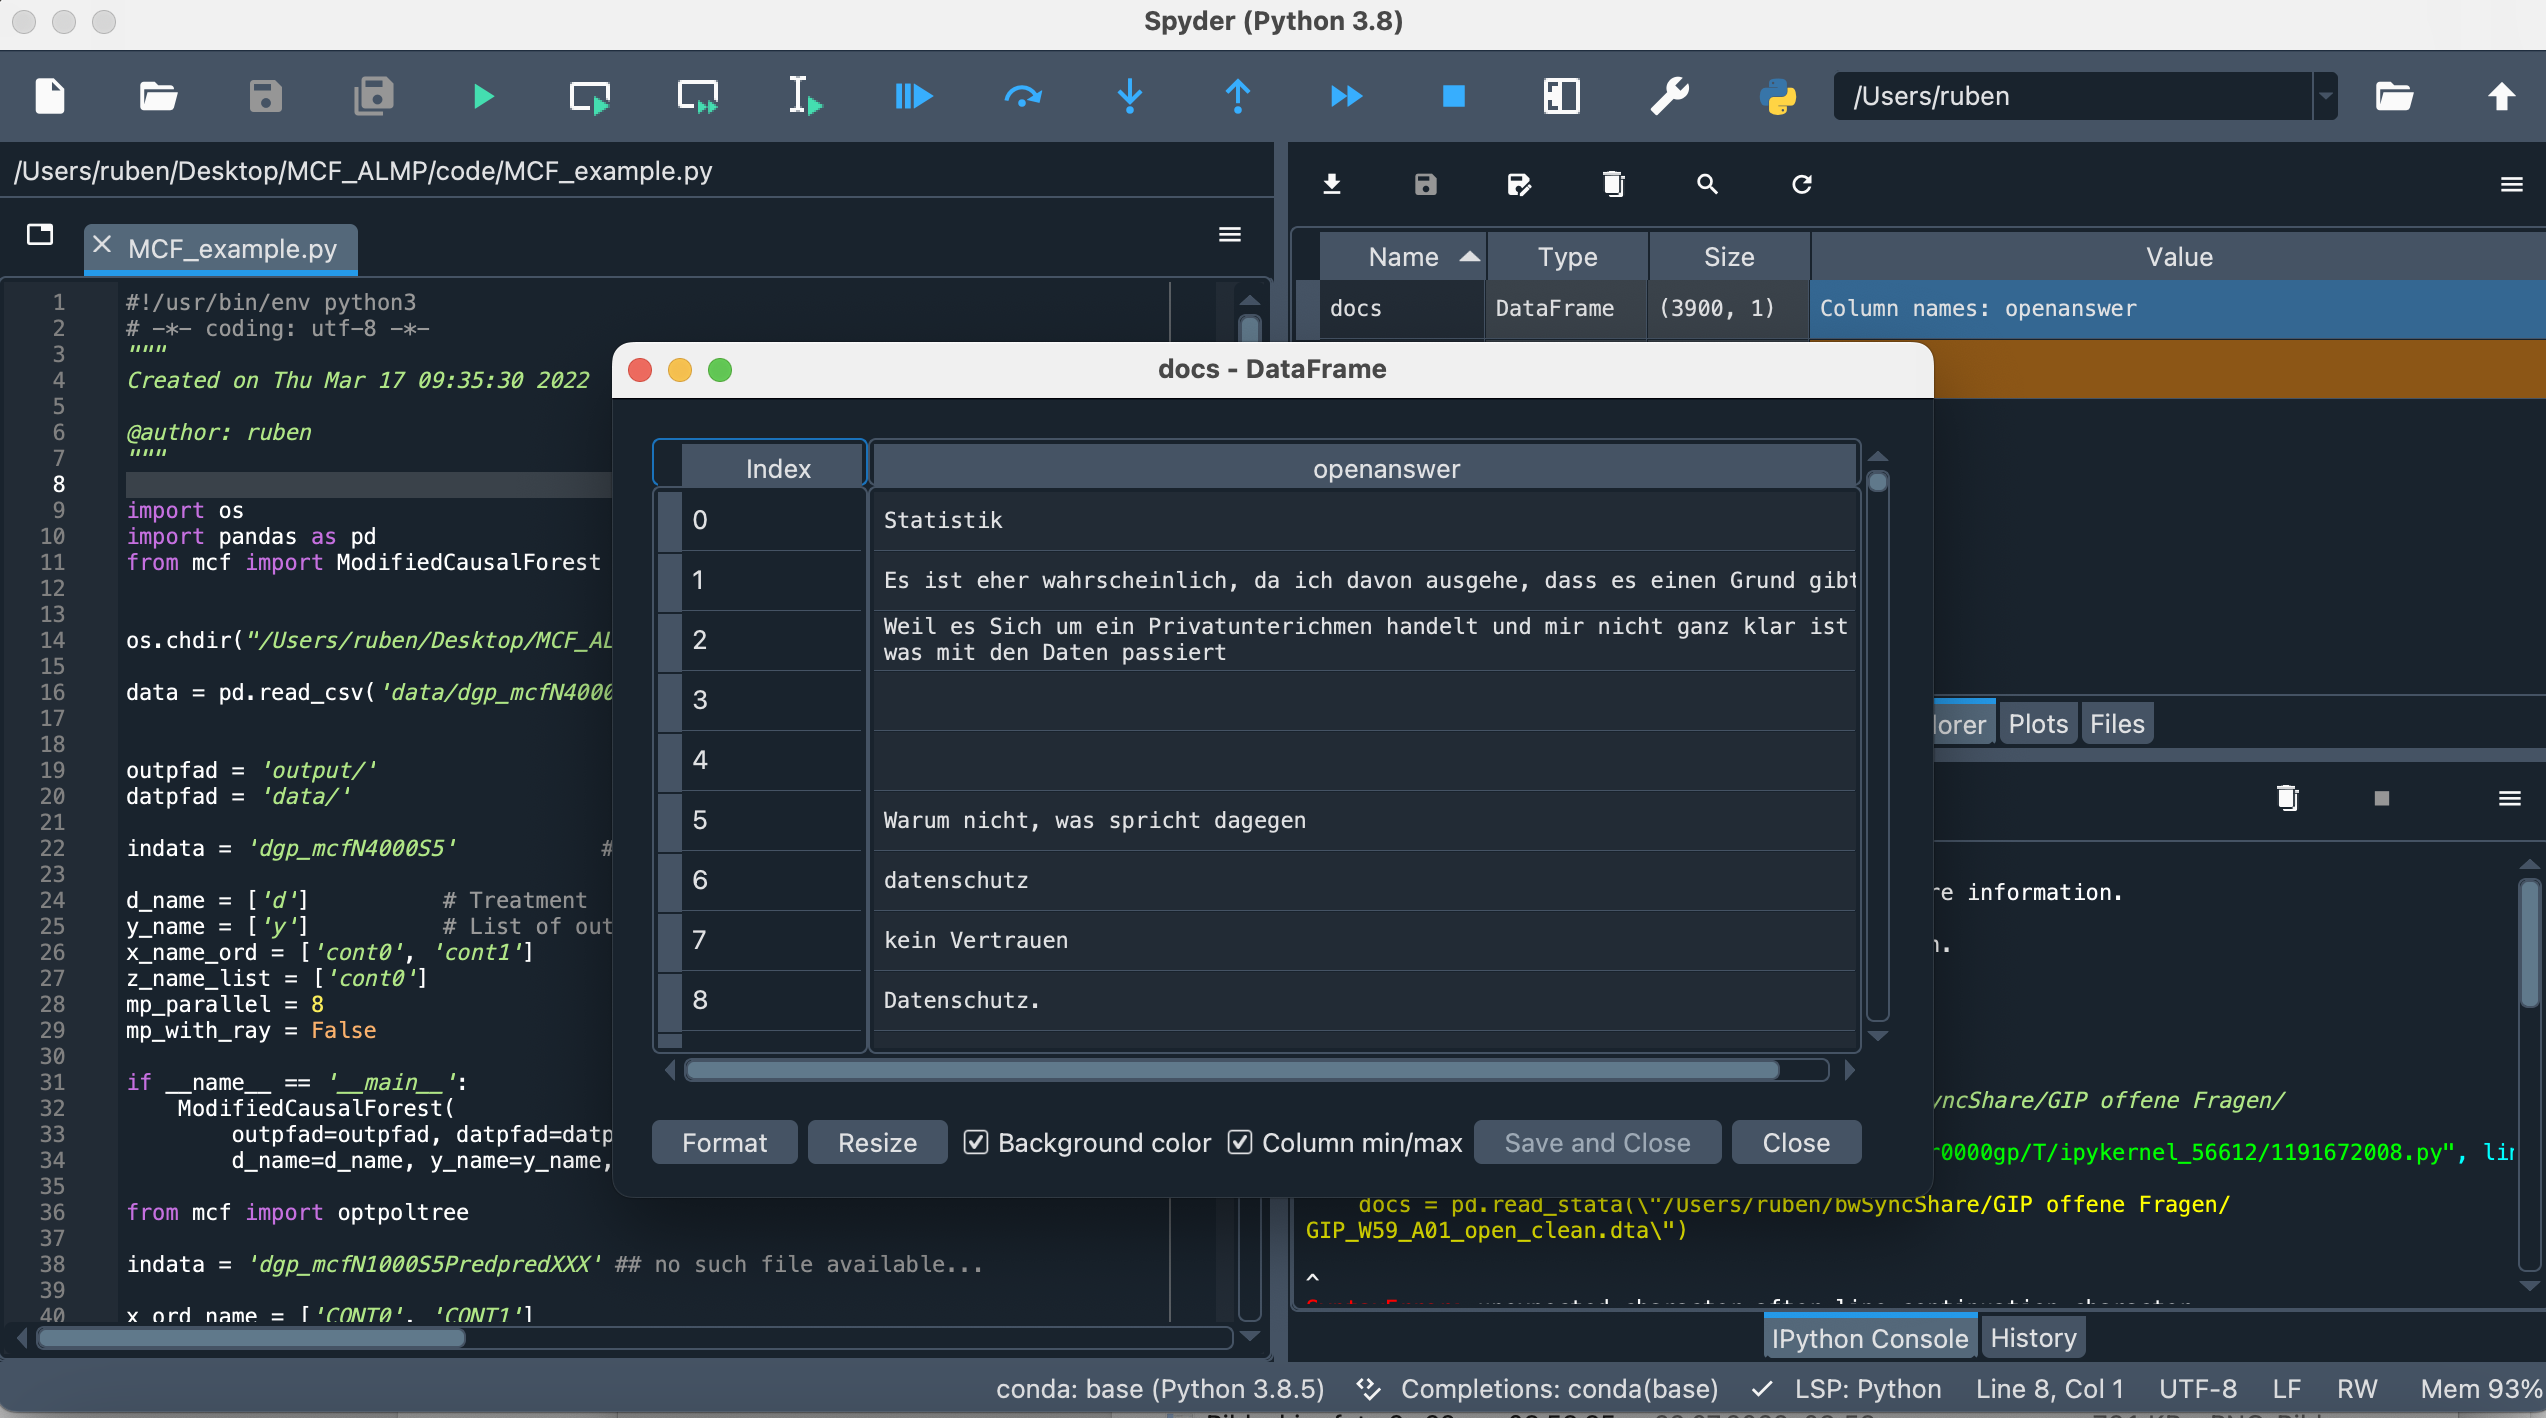
\includegraphics[scale=.28]{Day 1/Slides/LaTeX files/Spyder-2.png} \\
     \end{center}
\end{frame}

\begin{frame}{Jupyter Notebook}
    \small
    \begin{itemize}
        \item Web-based interactive computing environments
        \item Combine markdown with code, interactive cells, lots of exporting and publishing options
        \item Can run bash commands from within notebook using "!"
    \end{itemize}
    \begin{block}{Example: List installed packages using bash}
        !pip list
    \end{block}
    \begin{itemize}
        \item Magics (\% and \%\%) give additional cell functionality 
    \end{itemize}       

    \begin{block}{Example: Include HTML content in notebook}
        \%\%HTML
    \end{block}
    
\end{frame}

\begin{frame}{Jupyter Notebook}

   \begin{center}
       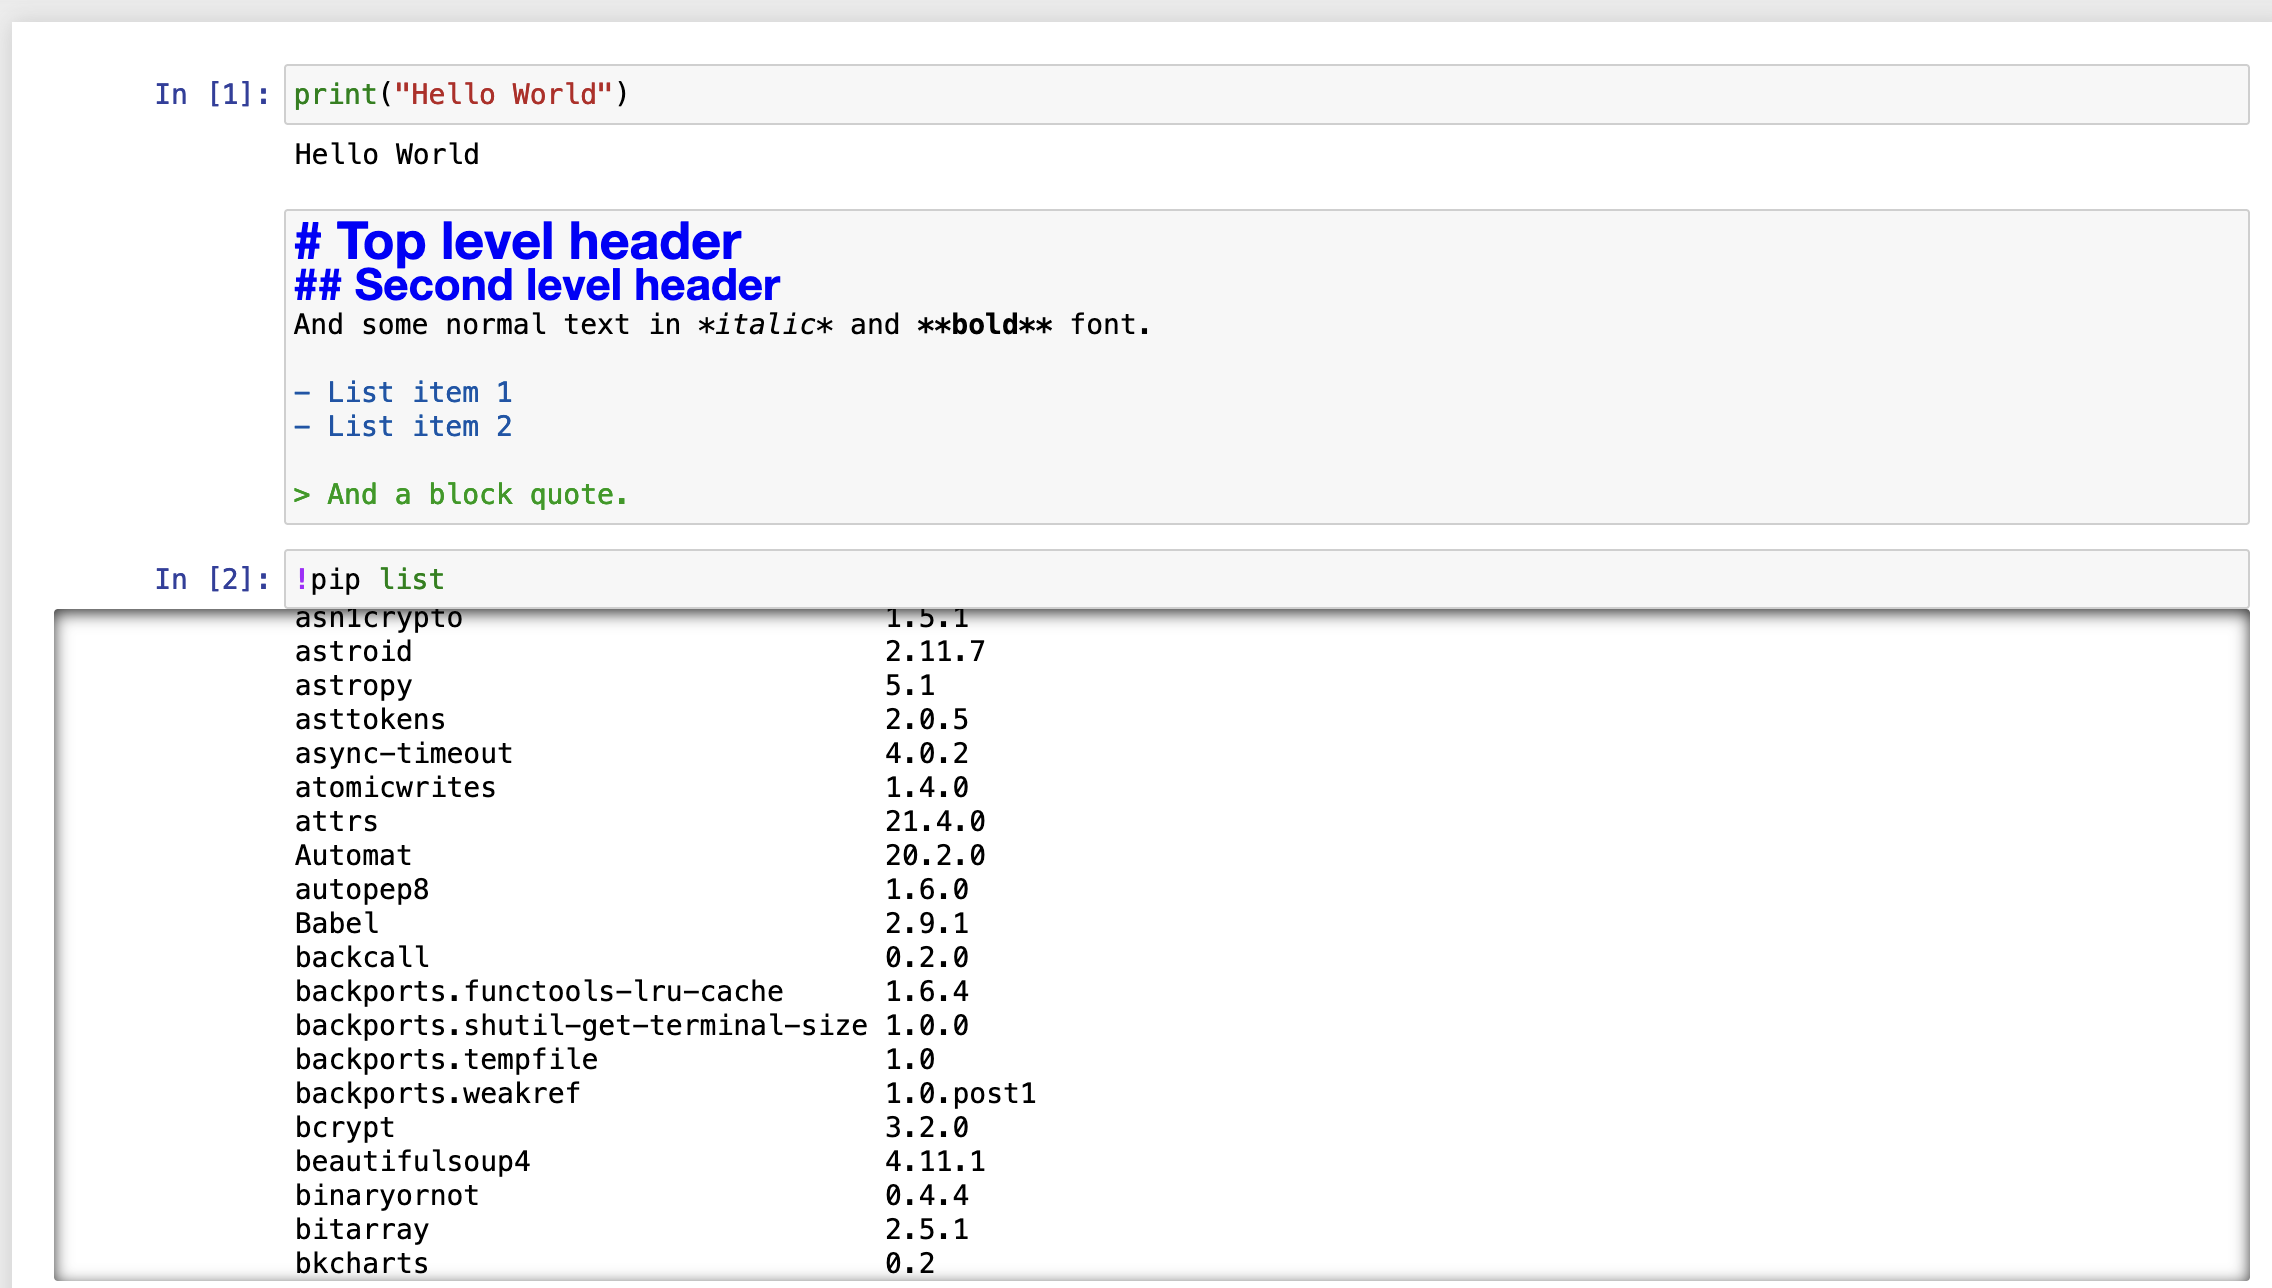
\includegraphics[scale=0.3]{Day 1/Slides/LaTeX files/Notebook2.png}
   \end{center}
    
\end{frame}

\begin{frame}{Jupyter Notebook}

   \begin{center}
       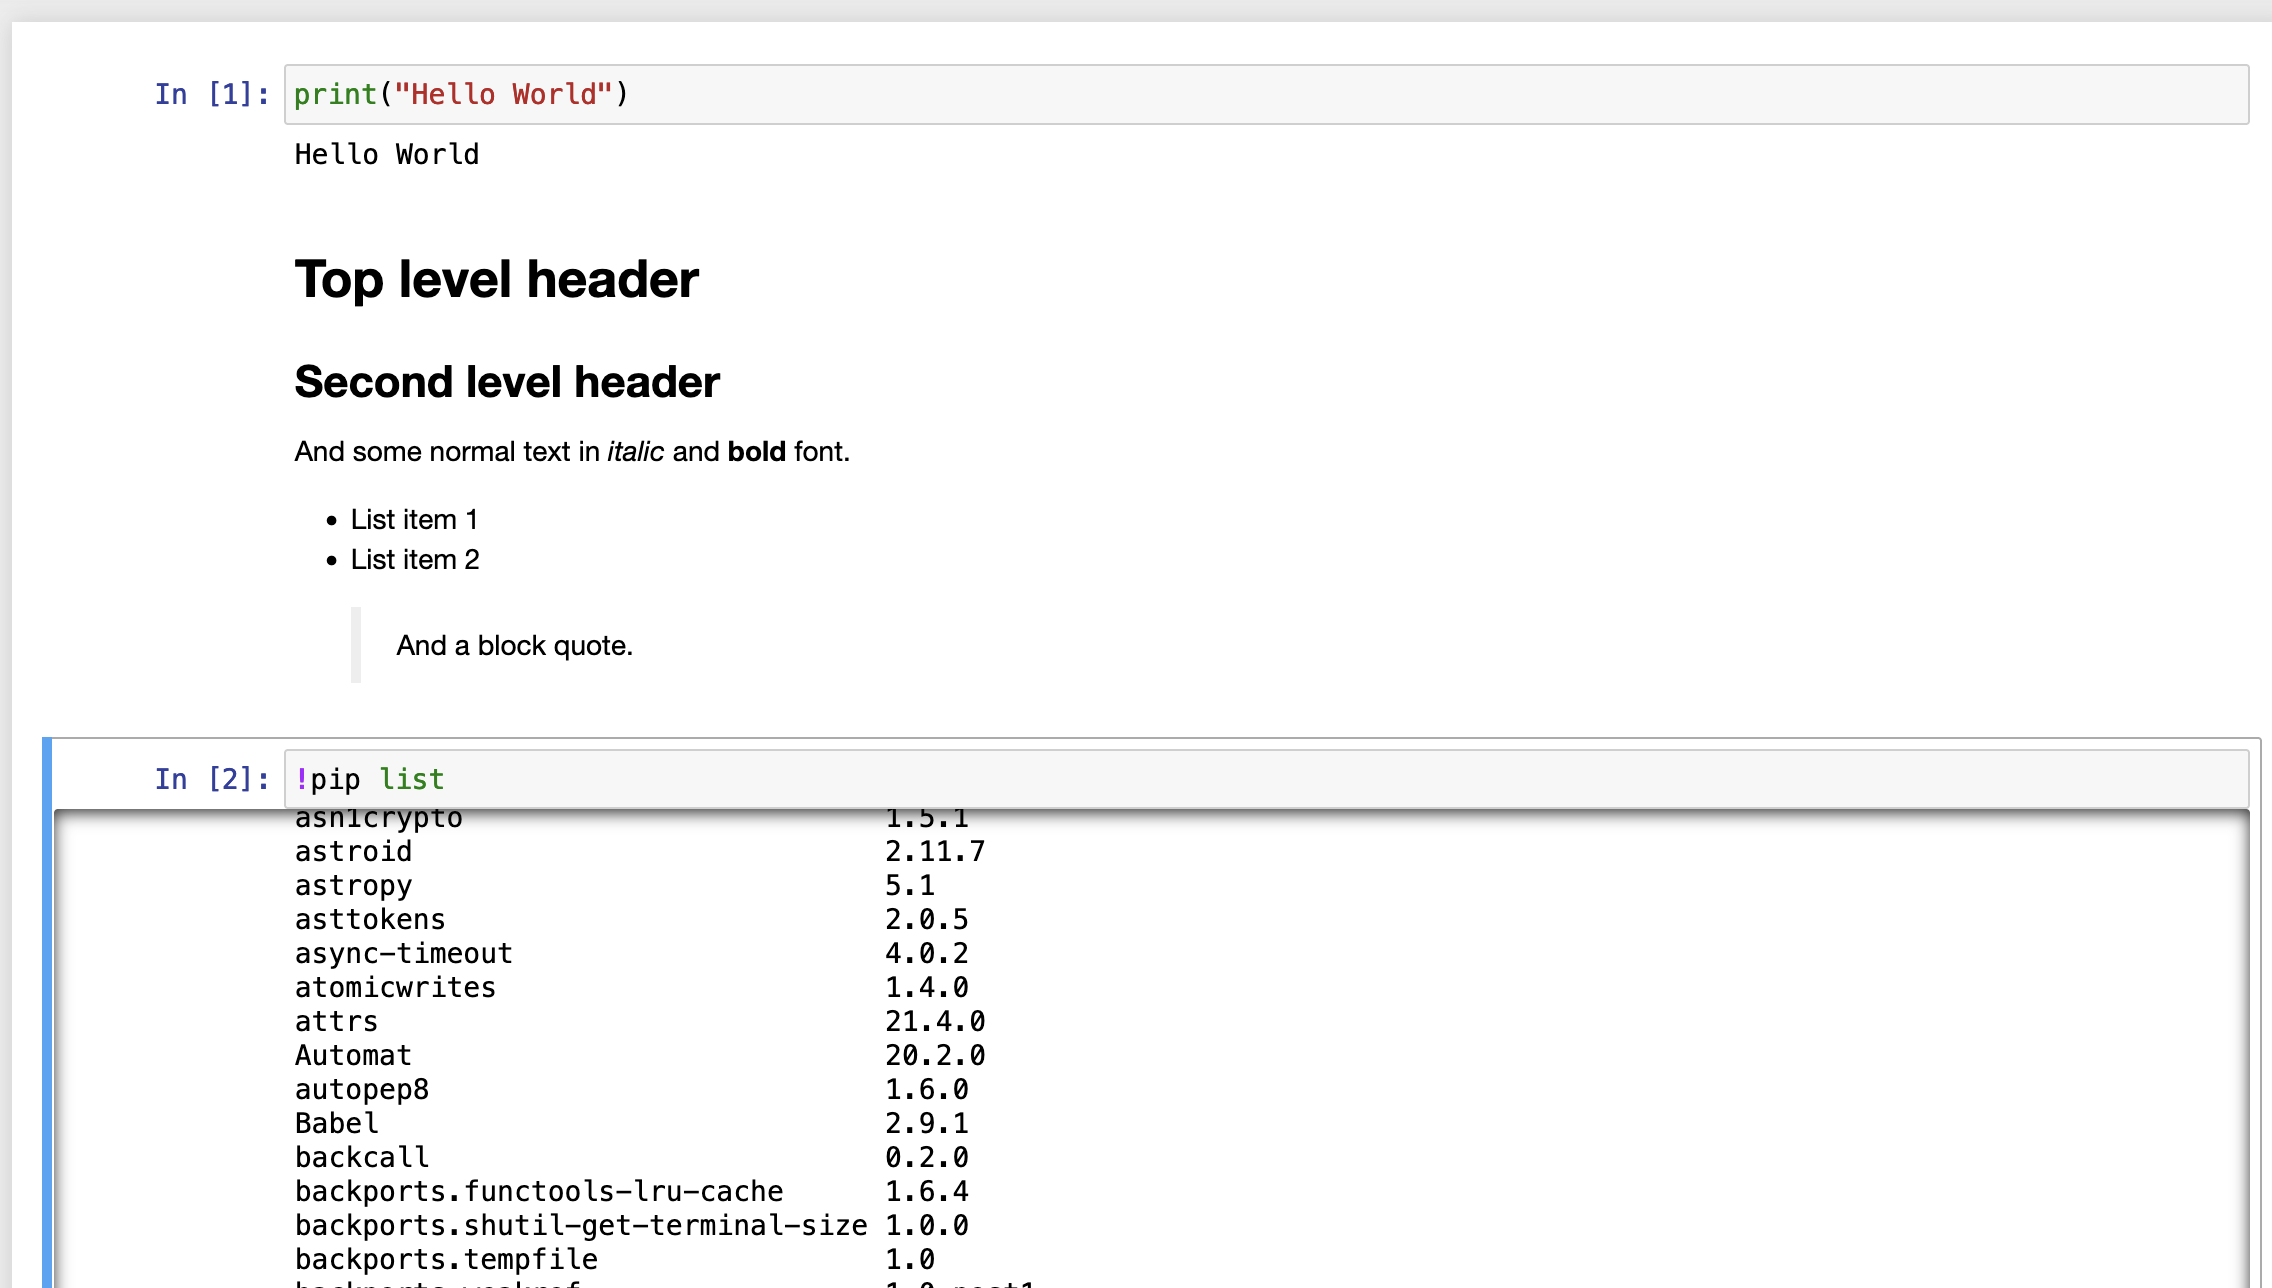
\includegraphics[scale=0.3]{Day 1/Slides/LaTeX files/Notebook3.png}
   \end{center}
    
\end{frame}

\begin{frame}{Jupyter Notebook}

   \begin{center}
       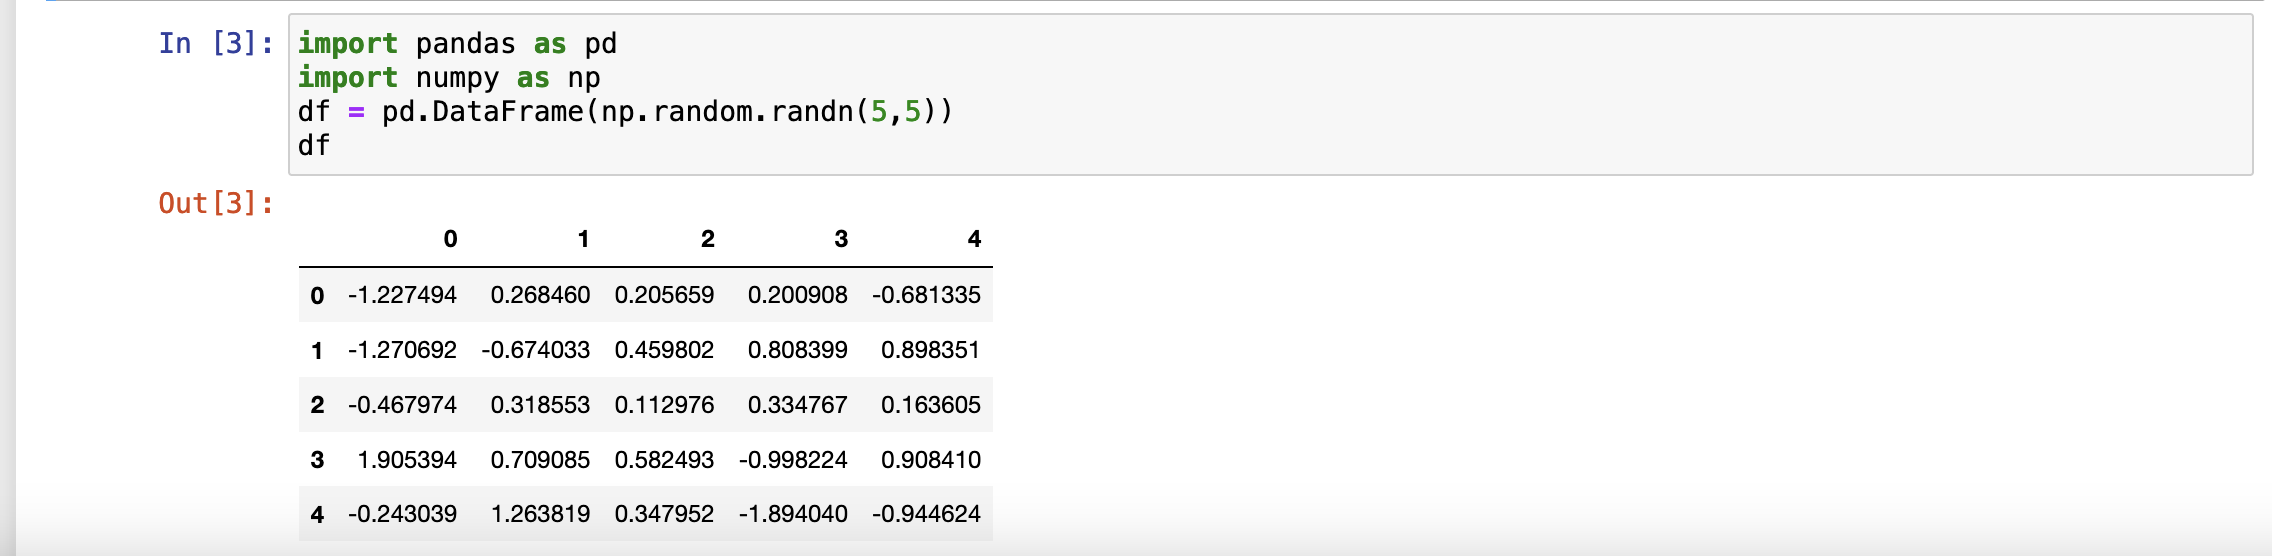
\includegraphics[scale=0.3]{Day 1/Slides/LaTeX files/Notebook1.png}
   \end{center}
    
\end{frame}

\begin{frame}{Jupyter Notebook}

   \begin{center}
       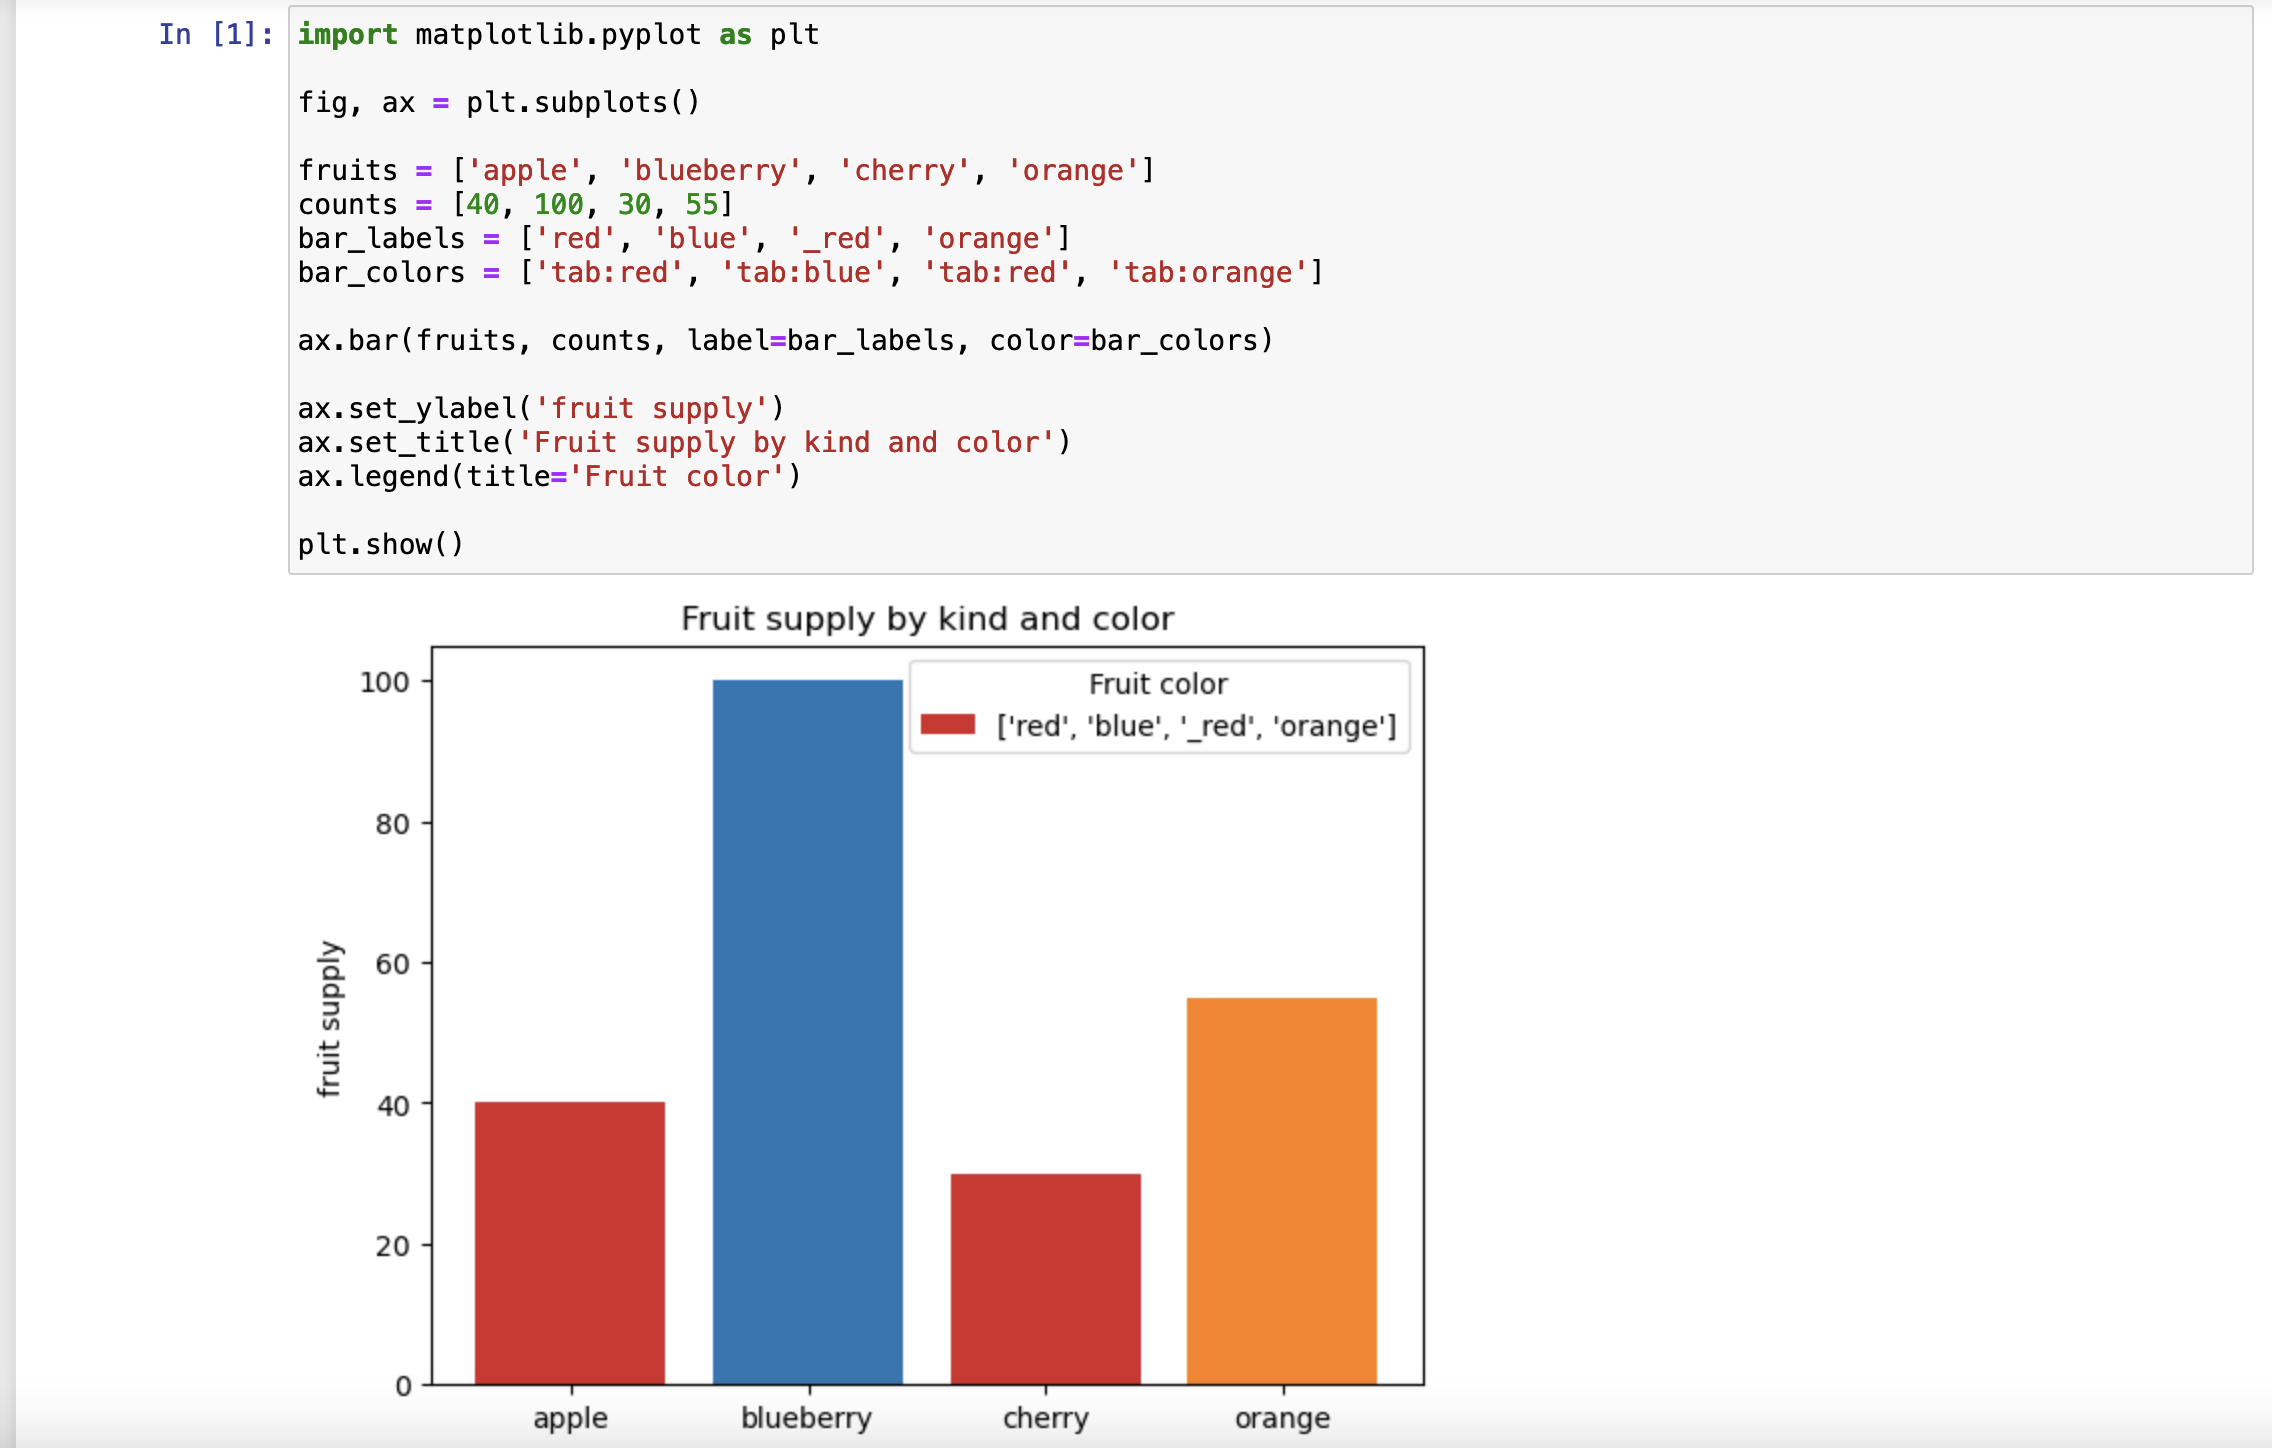
\includegraphics[scale=0.3]{Day 1/Slides/LaTeX files/Notebook4.png}
   \end{center}
    
\end{frame}


\begin{frame}{Google Colaboratory}
    \small
    \cemph{"Colab"}
    \begin{itemize}
        \item Web-based interactive computing environments
        \item Google account required
        \item Runs on Google hardware (including free GPU use)
        \item Powerful hardware available per premium plans
        \item Markdown-based text cells and code cells, magic commands, bash commands ("!"), R kernels available, \LaTeX, ...
        \item Load data from your Google Drive
        \item Pay attention when sharing colab notebooks
    \end{itemize}
    
    
\end{frame}

\begin{frame}{Google Colaboratory}
    \small
    \cemph{"Colab"} -- Downsides
    \begin{itemize}
        \item Lose data and results when runtime stops
        \item Uploaded files removed when session restarted, no persistent storage 
        \item Sensitive data? Sensitive code?
        \end{itemize}
    
    
\end{frame}

 	\section{Alternatives}
\begin{frame}{Reticulate}
    \begin{itemize}
        \item An R package that allows you to run Python code in R
        \item Requires miniconda or Anaconda installation
        \item Management of virtual environments and packages through conda
        \item Pro: Allows you to switch between R and Python code and access objects created in Python (e.g., data) in R
        \item Con: Environments and packages need to be managed through conda, troubleshooting can be more difficult
    \end{itemize}
\end{frame}

	\begin{frame}{rpy2}
  \begin{columns}
\begin{column}{0.5\textwidth}
    \begin{itemize}
        \item A Python library that allows you to run R code in Python
        \item You have to ‘translate’ R functions to call them from Python
        \item Alternatively, write and evaluate R code using \gemph{rmagic} in Jupyter Notebook (based on \textit{rpy2})
    \end{itemize}
\end{column}
\begin{column}{0.5\textwidth}  %%<--- here
    \begin{center}
      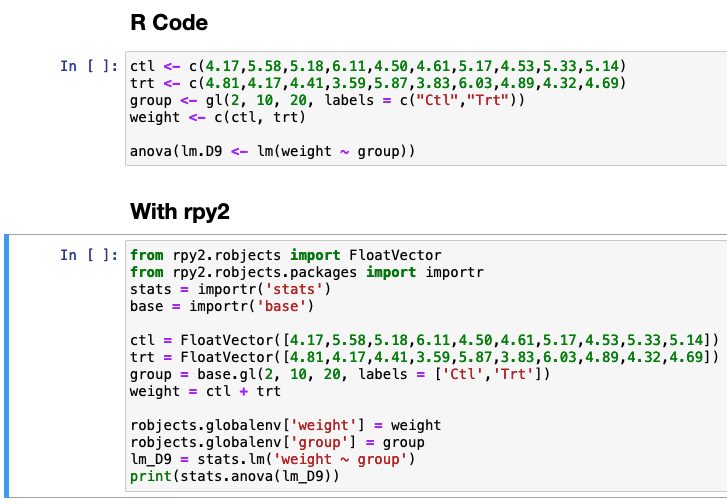
\includegraphics[scale=.28]{Day 1/Slides/LaTeX files/rpy2.png} 
     \end{center}
\end{column}
\end{columns}
  \end{frame}

\section{Further notes}
\begin{frame}{Naming conventions}
    \begin{itemize}
        \item A name can only consist of characters from three groups: digits (0-9), letters (a-z and A-Z), and underscores (\_)
        \item A name cannot start with a digit
        \item A name cannot coincide with one of Python’s reserved words, which have special meaning to Python, e.g., ...
        \begin{itemize}
            \item False, not, class, finally, is, return, None, continue, while, del, else, ...
        \end{itemize}
    \end{itemize}
\end{frame}

\begin{frame}{Indentation}
  \begin{columns}
\begin{column}{0.5\textwidth}
    \begin{itemize}
        \item Indentation: spaces at the beginning of a code line
        \item E.g., in R, indentation is for readability only, in Python it is very important
        \item Python uses indentation to indicate a block of code
        \item Number of spaces is up to you, but it has to be at least one and consistent
    \end{itemize}
\end{column}
\begin{column}{0.5\textwidth}  %%<--- here
    \begin{center}
      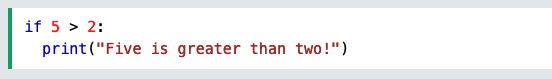
\includegraphics[scale=.28]{Day 1/Slides/LaTeX files/indentation_1.png}
      \vskip 1cm
      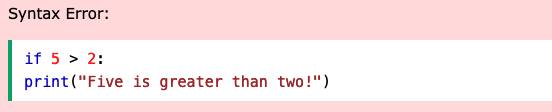
\includegraphics[scale=.28]{Day 1/Slides/LaTeX files/indentation_2.png}
     \end{center}
\end{column}
\end{columns}
    
\end{frame}

\begin{frame}{Importing and Using Packages}
  \begin{columns}
\begin{column}{0.5\textwidth}
    \begin{itemize}
        \item Depending on how you import a package, you will need to reference it when using a function
        \item Usually a good idea to use alternate names (e.g., pandas -> pd, numpy -> np)
        \item Can import submodules instead of whole packages
    \end{itemize}
\end{column}
\begin{column}{0.5\textwidth}  %%<--- here
    \begin{center}
      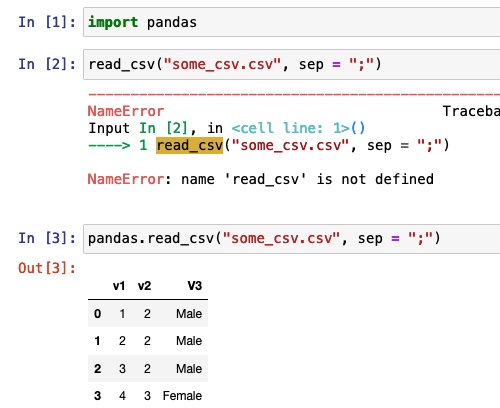
\includegraphics[scale=.28]{Day 1/Slides/LaTeX files/import_1.png}
      \vskip .5cm
      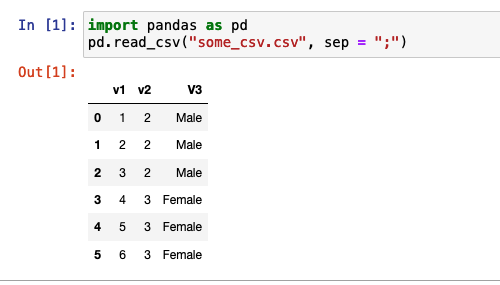
\includegraphics[scale=.28]{Day 1/Slides/LaTeX files/import_2.png}
      
     \end{center}
\end{column}
\end{columns}
    
\end{frame}


\begin{frame}{Importing and Using Packages}
  \begin{columns}
\begin{column}{0.5\textwidth}
    \begin{itemize}
        \item Depending on how you import a package, you will need to reference it when using a function
        \item Usually a good idea to use alternate names (e.g., pandas -> pd, numpy -> np)
        \item Can import elements of a package instead of whole packages
    \end{itemize}
\end{column}
\begin{column}{0.5\textwidth}  %%<--- here
    \begin{center}
      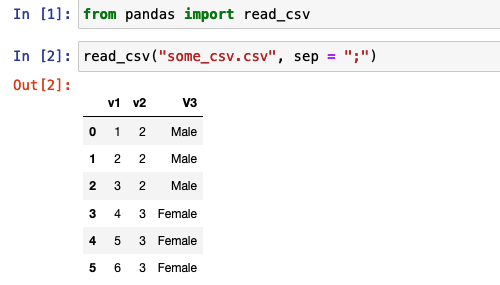
\includegraphics[scale=.28]{Day 1/Slides/LaTeX files/import_3.png}      
     \end{center}
\end{column}
\end{columns}
    
\end{frame}


 	\section{Additional Resources}
	\begin{frame}{Some Helpful Resources}
		\begin{itemize}
		    \item \href{https://www.freecodecamp.org/news/why-you-need-python-environments-and-how-to-manage-them-with-conda-85f155f4353c}{Virtual environments and managing them with conda}
            \item \href{https://www.youtube.com/watch?v=HW29067qVWk}{Jupyter Notebook tutorial}
            \item \href{https://www.youtube.com/watch?v=U3ByGh8RmSc}{reticulate}
            \item \href{https://rpy2.github.io/doc/latest/html/introduction.html}{rpy2}
            \item \href{https://datacamp.com}{Datacamp}
		\end{itemize}
	\end{frame}
	
	
	}
\end{document}